\documentclass{beamer}
\usepackage{graphicx}

\usetheme{Madrid}
\usecolortheme{default}

\title{Weather Forecasting}
\author{Jawad Ahmed 20P-0165}
\institute{National University of Computer and Emerging Sciences}
\date{\today}

\begin{document}

\begin{frame}
\titlepage
\end{frame}

\begin{frame}{Outline}
\tableofcontents
\end{frame}

\section{Research Problem}

\begin{frame}{Research Problem}
\begin{itemize}
\item Comparative Study of Statistical and Machine Learning Model
\item Weather Istanbul Data 2009-2019
\end{itemize}
\end{frame}


\section{Literature Review}

\begin{frame}{Literature Review}
\begin{itemize}
\item Previous research used ARIMA and ANFIS models
\item Weather Dataset Istanbul (2000-2008)
\item Limited Research on using ES and SVM model on more recent data
\end{itemize}
\end{frame}

\section{How AI is solving this Problem?}

\begin{frame}{How AI is solving this Problem?}
\begin{itemize}
\item Machine Learning Techniques
\item ARIMA
\item Exponential Smoothing
\item Support Vector Machine
\end{itemize}
\end{frame}

\section{Methodology}

\begin{frame}{Methodology}
 \begin{figure}
    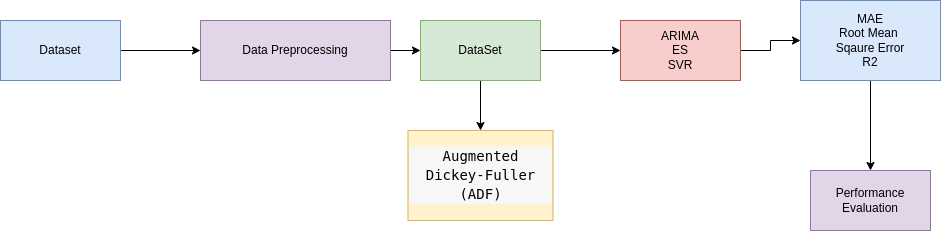
\includegraphics[width=\textwidth]{ai_class_project_methodolog.png}
    \caption{Methdology}
  \end{figure}
\end{frame}


\section{Results}

\begin{frame}{Results}
\begin{table}[h]
\centering
\small
\label{tab:my_table}
\begin{tabular}{|p{1.5cm}|p{1.5cm}|p{1.5cm}|p{1.5cm}|p{1.5cm}|}
\hline
Model & MAE & RMSE & R2 \\
\hline
ARIMA & 3.520 & 5.225 & -0.010 \\
ES & 9.304 & 9.576 & -2.39 \\
SVM & 2.000 & 4.570 & 0.23 \\
\hline
\end{tabular}
\end{table}
\end{frame}

\section{Benefits of this Research}

\begin{frame}{Benefits of this Research}
\begin{itemize}
\item Improve the accuracy of short-term long-term weather prediction
\item Streamlining Development Efforts
\item Time and Resource Efficiency
\end{itemize}
\end{frame}



\section{Future Work}

\begin{frame}{Future Work}
In the future work will apply these models:
\begin{itemize}
\item Neural Networks (e.g. LSTM, GRU) for time series prediction
\item Prophet, a forecasting library developed by Facebook for time series prediction
\end{itemize}
\end{frame}

\section{References}
\begin{frame}{References}
\begin{itemize}
\item [1] Box,G.E.P. and G.M.Jenkins, 1976.Time Series Analysis : Forecasting and Control. Holden Day Inc. San
Francisco,CA.
\end{itemize}

\end{frame}

\end{document}
